%%%%%%%%%%%%%%%%%%don't forget if needed %%%%%%%%%%%%%%%%%%%%%
%\section[toc version]{title version%
%              \sectionmark{head version}}
%\sectionmark{head version}
%%%%%%%%%%%%%%%%%%%%%%%%%%%%%%%%%%%%%%%%%%%%%%%%%%%%%%%%%%%%%%
\def\titcourt{Finite element method for the Navier-Stokes-Boussinesq equations using Newton algorithm}
\def\titlong{Finite element method for the Navier-Stokes-Boussinesq equations using Newton algorithm}
%%%%%%%%%%%%%%%%%%%%%%%%%%%%%%%%%%%%%%%%%%%%%%%%%%%%%%%%%%%%%%%%
\chapter[\titlong]{\titlong%
              \chaptermark{\titcourt}}
\chaptermark{\titcourt}
\label{chap-FEM}
%%%%%%%%%%%%%%%%%%%%%%%%%%%%%%%%%%%%%%%%%%%%%%%%%%%%%%%%%%%%%%%%
%%%%%%%%%%%%%%%%%%%%%%%%%%%%%%%%%%%%%%%%%%%%%%%%%%%%%%%%%%%%%%%%

%\section{Numerical method}\label{sec: num meth}

This chapter sets the numerical algorithm for solving the system of equation described previously in chapter \ref{chap-NSB} for both two and three-dimensional configurations.
The finite element method and the Newton algorithm are presented first in detail.
The accuracy of the developed method is then assessed with some basic theoretical test for two-dimensional configurations.
Finally, the domain decomposition method for the three-dimensional configuration is presented with a strong scalability analysis.

\section{Motivation for the choice of the numerical method}
Aside from the non-linear convection terms in the momentum and the energy eqs. (\ref{eq-qmvt})-(\ref{eq-energ}), a further difficulty arise from the non-linearity introduced by the source term $\partial (CS)/\partial t$ in eq. (\ref{eq-energ}).
In many in-house or commercial codes used to simulate phase-change problems (ANSYS CFX, Fluent, etc.),
finite difference (FD) or finite volume (FV) methods are used in most of the time with a fixed-mesh approach.
Accurate simulations are therefore carried out by increasing considerably the mesh resolution in the whole domain, increasing consequently dramatically the computational time.
At the example of \cite{voller1996cyclic} who used insufficient grid resolution to compute the melting of a gallium, \cite{wang2010numerical} had to consider thinner mesh resulting on an increase by a factor of three the total mesh number to capture correctly the boundary layer structures. 

Our choice for the finite element (FE) methods is motivated by its capability to adapt dynamically the mesh and to deal with several geometrical domain.
The adaptive capabilities of FE discretization by applying finer mesh where sharp phenomena takes place (solid-liquid interfaces, boundary layers, recirculation zones, ...) and coarser mesh elsewhere (in the solid, in the bulk of the fluid region where the gradient are lower than the boundary layer region, ...) is helpful to reduce the degree of freedom involved in the numerical resolution and thus reduce the computational time.
We use a finite-element method that was implemented using the open-source software FreeFem++ \citep{freefem,hecht-2012-JNM}, using a large variety of triangular finite elements  to solve partial differential equations. 

FreeFem++  is an integrated product with its own high level programming language and a syntax close to mathematical formulations, making the implementation of numerical algorithms very easy. Among the numerous numerical tools offered by FreeFem++, the use of the powerful mesh adaptivity function proved mandatory in this study to obtain accurate results within reasonable computational time.
The numerical code was optimized to afford the mesh refinement every time step:  the mesh density was increased around  the phase change interfaces,  offering an optimal resolution of the large gradients of all regularized functions ($S, K, C, \varphi$), while  the mesh was de-refined (larger triangles) in the solid part, where a coarser mesh could be used. A simulation using a globally refined mesh would require a prohibitive computational time for an equivalent accuracy of the melting front resolution. Similar algorithms based on FreeFem++  were successfully used for solving different systems of equations with locally sharp variation of the solution, such as Gross-Pitaevskii equation \citep{dan-2010-JCP,dan-2016-CPC} or  Laplace equations with nonlinear source terms \citep{dan-2013-AMM}. 

The space discretization is based on Taylor-Hood finite elements, approximating  the velocity with $P_{2}$ Lagrange finite elements (piecewise quadratic), and the
the pressure with the $P_{1}$ finite elements (piecewise linear). The temperature and the enthalpy are discretized using $P_2$ finite elements.  
This discretization is second order accurate in space.
We also use a second order accurate discretization in time.
\cite{aldbaissy2018full} have compared analytically and numerically the first and second order discretization of the time-dependent Boussinesq problem, and have concluded that the second order scheme is much better than the first order in terms of CPU time with the same precision.
A fully implicit backward second order scheme (BDF2 or GEAR) is employed in the present study. The time derivative of a variable $\phi$ is approximated  by:
\begin{equation}	
\label{eq-Gear}
	\frac{d\phi}{dt} \simeq \frac{3\phi^{n+1} - 4\phi^{n}+ \phi^{n-1}}{2\delta t},
\end{equation}
computing the solution $\phi^{n+1}$ at time  $t_{n+1}=(n+1) \delta t$ by using two previous states ($\phi^{n}, \phi^{n-1}$). We use this scheme to advance in time both velocity ($\phi=\vec{u}$) and temperature fields  ($\phi=\theta$).  The other terms in eqs. (\ref{eq-qmvt})-(\ref{eq-energ}) are treated implicitly (\ie taken at time $t_{n+1}$). The resulting non-linear equations are solved using a Newton algorithm. 
Some authors used a Richardson extrapolation \citep{Belhamadia2012,wang2010numerical} in the momentum equation by extrapolating U from previous time steps.
We have tested this approach but the results exhibit less accurate solutions and the computations requests small $\delta t$.
In addition, a projection algorithm with an explicit discretization of the Navier-Stokes-Boussinesq equations was also tested, using the Adams-Bashforth and Crank-Nicolson second order scheme.
The main drawback is the very small $\delta t$ ($\sim 10^{-6}$ vs $10^{-1}$ for the fully implicit discretization) needed to ensure convergence at each time steps.
A last alternative for the treatment of non-linear terms in the momentum equation is offered by the characteristics Galerkin method \cite{Pironneau92}.
This method will be discussed in detail in sec. \ref{sec-charac-FreeFem}.

Finally, a supplementary difficulty comes from the one-domain method which need techniques to bring the velocity to zero in the solid region.
The switch-off technique, the variable viscosity approach and the Carman-Kozeny penalty term are the most used in the literature.
The physical meaning of the variable viscosity formulation and the Carman-Kozeny penalty term is fundamentally different.
The Carman-Kozeny approach considers the mushy zone as a porous media, i.e the solid is stationary and the liquid flows through the porous structures, 
while the variable viscosity formulation treats the mushy zone as a mixture of solid crystals and liquid, permitting thus a movement of both the solid and the liquid.
The $\mu$-based method was investigated by \cite{dan-2014-JCP} and the Carman-Kozeny penalty method is investigated in the present work.
We note however that techniques in FV methods based on the modification of the numerical algorithm by cutting-off the velocity in the solid by a relaxation scheme also exists.

\newpage
\section{Finite element algorithm} \label{sec-FE-algo}

Finite-element methods for solving Navier-Stokes type systems of equations  are generally based on a separate discretization of the temporal derivative (using finite difference, splitting or characteristics methods) and the generalization of the Stokes problem for the resulting system \citep{Temam,GRaviart,Quarteroni}. We use the second-order implicit finite-difference discretization (\ref{eq-Gear}) of the temporal derivative and obtain the time semi-discretization of the single-domain model (\ref{eq-qmvt})-(\ref{eq-energ}):
\begin{eqnarray} \label{eq-time-disc1}
\nabla\cdot \vec{u}^{n+1} + {\gamma} p^{n+1} &=& 0, \\ %\nonumber
\frac{3}{2} \frac{\vec{u}^{n+1}}{\delta t} +(\vec{u}^{n+1}\cdot\nabla) \vec{u}^{n+1} +\nabla p^{n+1} 
- {\frac{1}{Re} \nabla^2 \vec u^{n+1}}  & & \\ \nonumber 
- A(\theta^{n+1})\vec u^{n+1}- f_B(\theta^{n+1}) \, \vec{e}_y &=&  \\ \nonumber
2 \frac{\vec{u}^{n}}{\delta t}-\frac{\vec{u}^{n-1}}{2\delta t},\\ \label{eq-time-disc3}
\frac{3}{2} \frac{\theta^{n+1} + S(\theta^{n+1})}{\delta t} +
\nabla\cdot\left(\vec{u}^{n+1} \theta^{n+1}\right)
- \nabla \cdot\left( \frac{K}{RePr} \nabla \theta^{n+1} \right) &=& \\  \nonumber
2\frac{ \theta^{n} + S(\theta^{n})}{\delta t}-\frac{ \theta^{n-1} + S(\theta^{n-1}) }{2\delta t}.
\end{eqnarray}
The penalty parameter $\gamma$ takes very low values ($\gamma=10^{-7}$)  to ensure a pressure field with zero average and, at the algebraic level, fulfill the diagonal of the pressure term.  
This system of non-linear equations is solved at time  $t_{n+1}=(n+1) \delta t$, using two  previous states at $t_{n}$ and $t_{n-1}$.

The space discretization of variables over the domain $\Omega=[0,1]^2$ uses a finite-element method based on a weak formulation of the system of eqs. (\ref{eq-time-disc1})-(\ref{eq-time-disc3}). 
We consider homogeneous Dirichlet boundary conditions for the velocity, \ie $\vec{u}=0$ on $\pl \Omega$, and set the classical Hilbert spaces for the velocity and pressure:
\begin{equation}
\vec{V}=V\times V, \, V=H^1_0(\Omega), \quad Q=\left\{q\in L^2(\Omega)\left|\; \int_{\Omega}q=0\right.\right\}
\end{equation}
Following the generalization of the Stokes problem \citep{Temam,GRaviart,Quarteroni}, the variational formulation of the system  (\ref{eq-time-disc1})-(\ref{eq-time-disc3}) can be written as: find $(\vec{u}^{n+1}, p^{n+1}, \theta^{n+1}) \in \vec{V}\times Q\times V$, such that:
\begin{eqnarray}
\label{eq-weak-all}
b\left(\vec{u}^{n+1}, q\right) - \gamma (p^{n+1},q)&=& \\ \nonumber
0, \, \forall \, q \in Q \\ %\nonumber
\frac{3}{2 \delta t} \left(\vec{u}^{n+1},\vec{v}\right) + c\left(\vec{u}^{n+1} ; \vec{u}^{n+1}, \vec{v} \right) +
{a\left(\vec{u}^{n+1}, \vec{v}\right)} & &\\ \nonumber
- (A(\theta^{n+1}) \, \vec u^{n+1},\vec v)+ b\left(\vec{v}, p^{n+1}\right)
- {\left(f_B(\theta^{n+1}) \, \vec{e}_y,\vec{v}\right)}
&=& \\ \nonumber
\frac{2}{\delta t} \left(\vec{u}^{n},\vec{v}\right) 
- \frac{1}{2 \delta t} \left(\vec{u}^{n-1},\vec{v}\right), \, \forall \, \vec{v} \in \vec{V}\\ \label{eq-weak-energy}  %\nonumber
\frac{3}{2 \delta t} \left(\theta^{n+1} + S(\theta^{n+1}), \phi\right)
+\left(\vec{u}^{n+1} \cdot \nabla \theta^{n+1} , \phi
\right) +
\left( \frac{K}{Re Pr} \nabla \theta^{n+1}, \nabla \phi \right) &=& \\  \nonumber
\frac{2}{\delta t} \left( \theta^{n}+S(\theta^n), \phi\right)
- \frac{1}{2 \delta t} \left( \theta^{n-1}+S(\theta^{n-1}), \phi\right),\, \forall \, \phi \in V,
\end{eqnarray}
where {$(u , v)=\int_{\Omega} u\cdot v$} denotes the scalar product in $L^2(\Omega)$ or $\left(L^2(\Omega)\right)^2$; the bilinear forms $a, b$ and trilinear form $c$ are defined as \cite{GRaviart,Quarteroni}:
\begingroup \small{
	\begin{eqnarray*}\nonumber
		a: \vec{V} \times \vec{V} \rightarrow \R, & & {a(\vec{u},\vec{v})= \int_{\Omega}  
			 \vec{D}(\vec{u}) : \vec{D}(\vec{v}) = \int_{\Omega}   \sum_{i,j=1}^2{D}_{ij}(\vec{u}) {D}_{ij}(\vec{v})},\\ 
		b: \vec{V} \times Q \rightarrow \R, & & b(\vec{u},q) = -\int_{\Omega}\nabla \cdot\vec{u}\, q =
		-\sum_{i=1}^2\int_{\Omega}\pl_i u_i\cdot q, \\ \nonumber
		c: \vec{V} \times \vec{V} \times \vec{V} \rightarrow \R, & & c(\vec{w}; \vec{z}, \vec{v})=\int_{\Omega} \left[\left(\vec{w} \cdot \nabla\right) \vec{z}\right] \cdot\vec{v}
		=\sum_{i,j=1}^2\int_{\Omega} w_j (\pl_j z_i) v_i,
		\label{eq-biforms}
	\end{eqnarray*}
}
$\vec D(\vec u) = (1/2)\left( \nabla \vec u + \nabla \vec u^T \right)$ is the rate of strain symmetric tensor with components
$D_{ij}(\vec u) = (1/2) \left( \partial u_i/ \partial x_j + \partial u_j/ \partial x_i \right) $.

The system of non-linear eqs. (\ref{eq-weak-all}) - (\ref{eq-weak-energy}) is solved using a Newton method. To advance the solution from time $t_n$ to $t_{n+1}$, we start from an initial guess $w_0 = (\vec{u}^{n}, p^{n}, \theta^{n})$ (which is the solution at $t_n$), and construct the Newton sequence $w_k = (u_k, p_k, \theta_k)$ by solving for each inner iteration $k$:
\begin{equation}
D_w{\cal F} (w_k ) w_{k+1} = D_w{\cal F}(w_k) w_k -  {\cal F}(w_k).
\label{eq-newton-w}
\end{equation}
$D_w{\cal F}$ is the linear operator representing the differential of $\cal F$.
Eq. (\ref{eq-newton-w}) can be rewritten as follow when applied to the discretized equation, in which eqs. (\ref{eq-weak-all}) - (\ref{eq-weak-energy}) are regarded as ${\cal F}(w) = 0$:
\begingroup \small{
	\begin{eqnarray} \label{eq-newton-C1}
	b\left(\vec{u}_{k+1}, q\right) - \gamma (p_{k+1},q) &=& 0, \\ %\nonumber
	\frac{3}{2 \delta t} \left(\vec{u}_{k+1},\vec{v}\right)
	+ c\left(\vec{u}_{k+1} ; \vec{u}_{k}, \vec{v} \right)
	&+& c\left(\vec{u}_{k} ; \vec{u}_{k+1}, \vec{v} \right)\\ \nonumber
	+ 
	a\left( \vec{u}_{k+1}, \vec{v}\right)
	- \left(\frac{d A}{d\theta}(\theta_k)\, \theta_{k+1} \, \vec{u}_k, \vec{v}\right)
	&-& \left(A(\theta_k) \, \vec{u}_{k+1}, \vec{v}\right) + b\left(\vec{v}, p_{k+1}\right)  \\ \nonumber
	- {\left(\frac{df_B}{d\theta}(\theta_k)\, \theta_{k+1} \, \vec{e}_y, \vec{v}\right)} &=&  
	\frac{1}{\delta t} \left( 2 \vec{u}^n - \frac{1}{2} \vec{u}^{n-1},\vec{v}\right) \\ \nonumber
	+ c\left(\vec{u}_k ; \vec{u}_{k}, \vec{v} \right) 
	&-& \left(\frac{d A}{d\theta}(\theta_k)\, \theta_{k} \, \vec{u}_k, \vec{v}\right), \,\,\, \\  %\nonumber
	\frac{3}{2\delta t} \left(\theta_{k+1} + \frac{dS}{d\theta}(\theta_k)\, \theta_{k+1}, \phi\right)
	+\left(\vec{u}_{k} \cdot \nabla \theta_{k+1} , \phi  \right)
	&+& \left( \vec{u}_{k+1} \cdot \nabla  \theta_k , \phi \right) \\ \nonumber
	+ \left( \frac{K}{Re Pr} \nabla \theta_{k+1}, \nabla \phi \right) 
	&=&
	\frac{2}{\delta t} \left(\theta^n + S(\theta^n) , \phi\right)  \\ \nonumber
	+\left(\vec{u}_{k} \cdot \nabla  \theta_k, \phi \right)
	+ \frac{3}{2 \delta t} \left(\frac{dS}{d\theta}(\theta_k)\, \theta_{k}  - S(\theta^n) ,\, \phi\right) 
	&-& \frac{1}{2 \delta t} \left(\theta^{n-1} + S(\theta^{n-1}),\, \phi\right).\,\,\,
	\end{eqnarray}
} \endgroup
We underline the fact that the Newton loop (following $k$) has to be iterated until convergence for each time step $\delta t$ following the algorithm:

\begin{equation} \label{eq-Newton-algo}
\begin{tabular}{||ll}
\multicolumn{2}{||l}{Navier-Stokes time loop following $n$}\\
\multicolumn{2}{||l}{set  $w_0=(\vec{u}^{n}, p^{n}, \theta^{n})$}\\
& \begin{tabular}[t]{||ll}
\multicolumn{2}{||l}{Newton iterations  following $k$}\\
&solve (\ref{eq-newton-C1}) to get $ \vec w_{k+1} $\\
\multicolumn{2}{||l}{stop when  $\| \vec w_{k+1} - \vec w_k \| < \xi_N$}
\end{tabular}\\
\multicolumn{2}{||l}{actualize $(\vec{u}^{n+1}, p^{n+1}, \theta^{n+1}) = w_{k+1}$}
\end{tabular}
\end{equation}
It is interesting to note that the previous system of equations depends only on $\vec{u}^n$, $\vec{u}^{n-1}$, $\theta^n$ and $\theta^{n-1}$ and is independent of $p^n$, the pressure being in this approach a Lagrange multiplier for the divergence free constraint. 

\section{Characteristics method for the convective terms} \label{sec-charac-FreeFem}

An alternative for the treatment of non-linear terms in the momentum equation is offered by the characteristics Galerkin method \cite{Pironneau92}. Defining the characteristic flow (passing at time $t$ through the point $\vec{x}$)
\begin{equation}
\left\{
\begin{array}{l}\vspace{0.2cm}
\ds\frac{\partial \vec{X} }{\partial \tau}(\tau, t, \vec{x})=\vec{u} (\tau,\vec{X} (\tau,t, \vec{x})), \quad \tau\in (0,t_{max})\\
\vec{X} (t, t, \vec{x}) = \vec{x},
\end{array}
\right.
\label{eq-charactD}
\end{equation}
one can express the substantial (total) derivative of any function $\Phi(t,\vec{x})$ as
\begin{equation}
\frac{D\Phi}{Dt}(t,\vec{x})=\left( \frac{\partial \Phi}{\partial
	t}+\vec{u}\cdot\nabla \Phi \right)(t,\vec{x})=\frac{\partial}{\partial
	t}\left(\Phi(\tau, \vec{X}(\tau,t, \vec{x}))\right)|_{\tau=t},
\end{equation}
and finally use the time discretization:
\begin{equation}
\left(\frac{D\Phi}{Dt}\right)^{n+1}(\vec{x})\approx\frac{\Phi^{n+1}(\vec{x})-\Phi^{n}\circ \vec{X}^n(\vec{x})}{\delta t},
\end{equation}
with $\vec{X}^n(\vec{x})$ a suitable approximation of $\vec{X}(t_n,t_{n+1},\vec{x})$, obtained by an integration back in time of (\ref{eq-charact}) from $t_{n+1}$ to $t_n$ for each grid point $\vec{x}$. The Galerkin characteristic method is implemented in Freefem++ as an operator computing $\Phi \circ \vec{X}^n$ for given mesh, convection velocity field and time step.

The weak formulation  (\ref{eq-weak-all}) becomes after using the characteristics method:
\begin{eqnarray}
\label{eq-charact}
b\left(\vec{u}^{n+1}, q\right) - \gamma (p^{n+1},q)&=& \\ \nonumber
0, \, \forall \, q \in Q \\ \nonumber
\frac{3}{2 \delta t} \left(\vec{u}^{n+1},\vec{v}\right) +
a\left(\vec{u}^{n+1}, \vec{v}\right) 
+ b\left(\vec{v}, p^{n+1}\right) 
- f_B(\theta^{n+1}) \left(\vec{e}_y,\vec{v}\right)
&=& \\ \nonumber
\frac{2}{\delta t} \left(\vec{u}^{n}\circ \vec{X}^n,\vec{v}\right) - \frac{1}{2 \delta t} \left(\vec{u}^{n-1}\circ \vec{X}^{n-1},\vec{v}\right), \, \forall \, \vec{v} \in \vec{V}\\  \nonumber
\frac{3}{2 \delta t} \left(\theta^{n+1}, \phi\right)  
+
\left( \frac{K}{\Prd} \nabla \theta^{n+1}, \nabla \phi \right) &=& \\ \nonumber
 \frac{2}{\delta t} \left(\theta^{n}\circ \vec{X}^n, \phi\right) -  \frac{1}{2 \delta t} \left(\theta^{n-1}\circ \vec{X}^{n-1}, \phi\right), \, \forall \, \phi \in V,
\end{eqnarray}
The system (\ref{eq-charact}) is then solved to advance the solution from $t_n$ to $t_{n+1}$ in one step. The drawback of the method is that it requires small time steps for accurately computing of the convection terms. 

 \section{Mesh adaptivity} \label{subs:FEadapt}

Mesh adaptivity by metric control is a standard function offered by FreeFem++ \citep{hecht-2012-JNM}. The key idea for the mesh adaptivity (see also \cite{hecht-2000-ijnmf,hecht-1997-aiaa,george-1998}) is to modify the scalar product used in an automatic mesh generator to evaluate distance and volume, in order to  construct equilateral elements according to a new adequate metric.  The scalar
product is based on the evaluation of the Hessian $\mathcal{H}$ of the variables of the problem. Indeed, for a $P_1$ discretization of a
variable $\chi$, the interpolation error is bounded by:
\begin{equation}
{\cal E } = |\chi - \Pi_h \chi |_0 \leq c \sup_{T\in \mathcal{T}_{h}} \sup_{x,y,z\in T}   |\mathcal{H}(x)|(y-z , y-z)
\label{eq1}
\end{equation}
where $\Pi_h \chi $ is the $P_1$ interpolate  of $\chi$, $ |\mathcal{H}(x)|$ is the  Hessian of $\chi$ at point $x$ after being made positive definite.
We can infer that, if we generate, using  a Delaunay procedure (e.g. \cite{george-1998}), a  mesh with edges close to the unit length  in the metric  $\mathcal{M} ={|\mathcal{H}| \over (c {\cal{E}})}$, the interpolation error ${\cal E}$ will be equally distributed over the edges $a_i$ of the mesh. More precisely, we have
\begin{equation}
{1 \over c {\cal E}} a_i^T {\cal M } a_i \le 1.
\end{equation}

The previous approach could be generalized for a vector variable $\chi=[\chi_1, \chi_2]$.
After computing the metrics $\mathcal{M}_{1}$ and $\mathcal{M}_{2}$ for each variable, we define a metric intersection  $\mathcal{M} = \mathcal{M}_{1} \cap \mathcal{M}_{2}$,
such that the unit ball of $\mathcal{M}$ is included in  the intersection of the two  unit balls  of metrics $\mathcal{M}_{2}$ and $\mathcal{M}_{1}$ (for details, see the  procedure defined in \cite{frey-george-1999}). 


%%%%%%%%%%%%%%%%%%%%%%%%%%%%%%%%%%%%%%%%%%%%%%%%%%%%%%%%%%%


\section{Accuracy and convergence} \label{subsec-conv}
We test the accuracy of our numerical method in this section.
Both space and time convergence orders are demonstrated by using the Burggraf flow and a manufactured solution defined by \cite{nourgaliev2016fully} for the incompressible Navier-Stokes equations.
The global error $ \| \varepsilon_h \|$ is defined as follows:

\begin{equation}
  \| \varepsilon_h \| = \| \Phi_e - \phi_h \|,
\end{equation}
where $\Phi_e$ is the exact solution and $\phi_h$ is the numerical solution.
Thus, by computing $\| \varepsilon_h \|$ for either different grids or different time steps, one can evaluate the convergence order $p$, since it is represented by the slope of the corresponding curve in logarithmic coordinates.

Computations are done for the convection of air, with a Rayleigh number $Ra = 10^6$ and a Prandtl number $Pr = 0.71$.

\subsection{Burggraf flow} \label{subsub-conv-burg}

\begin{figure}
	\begin{center}
		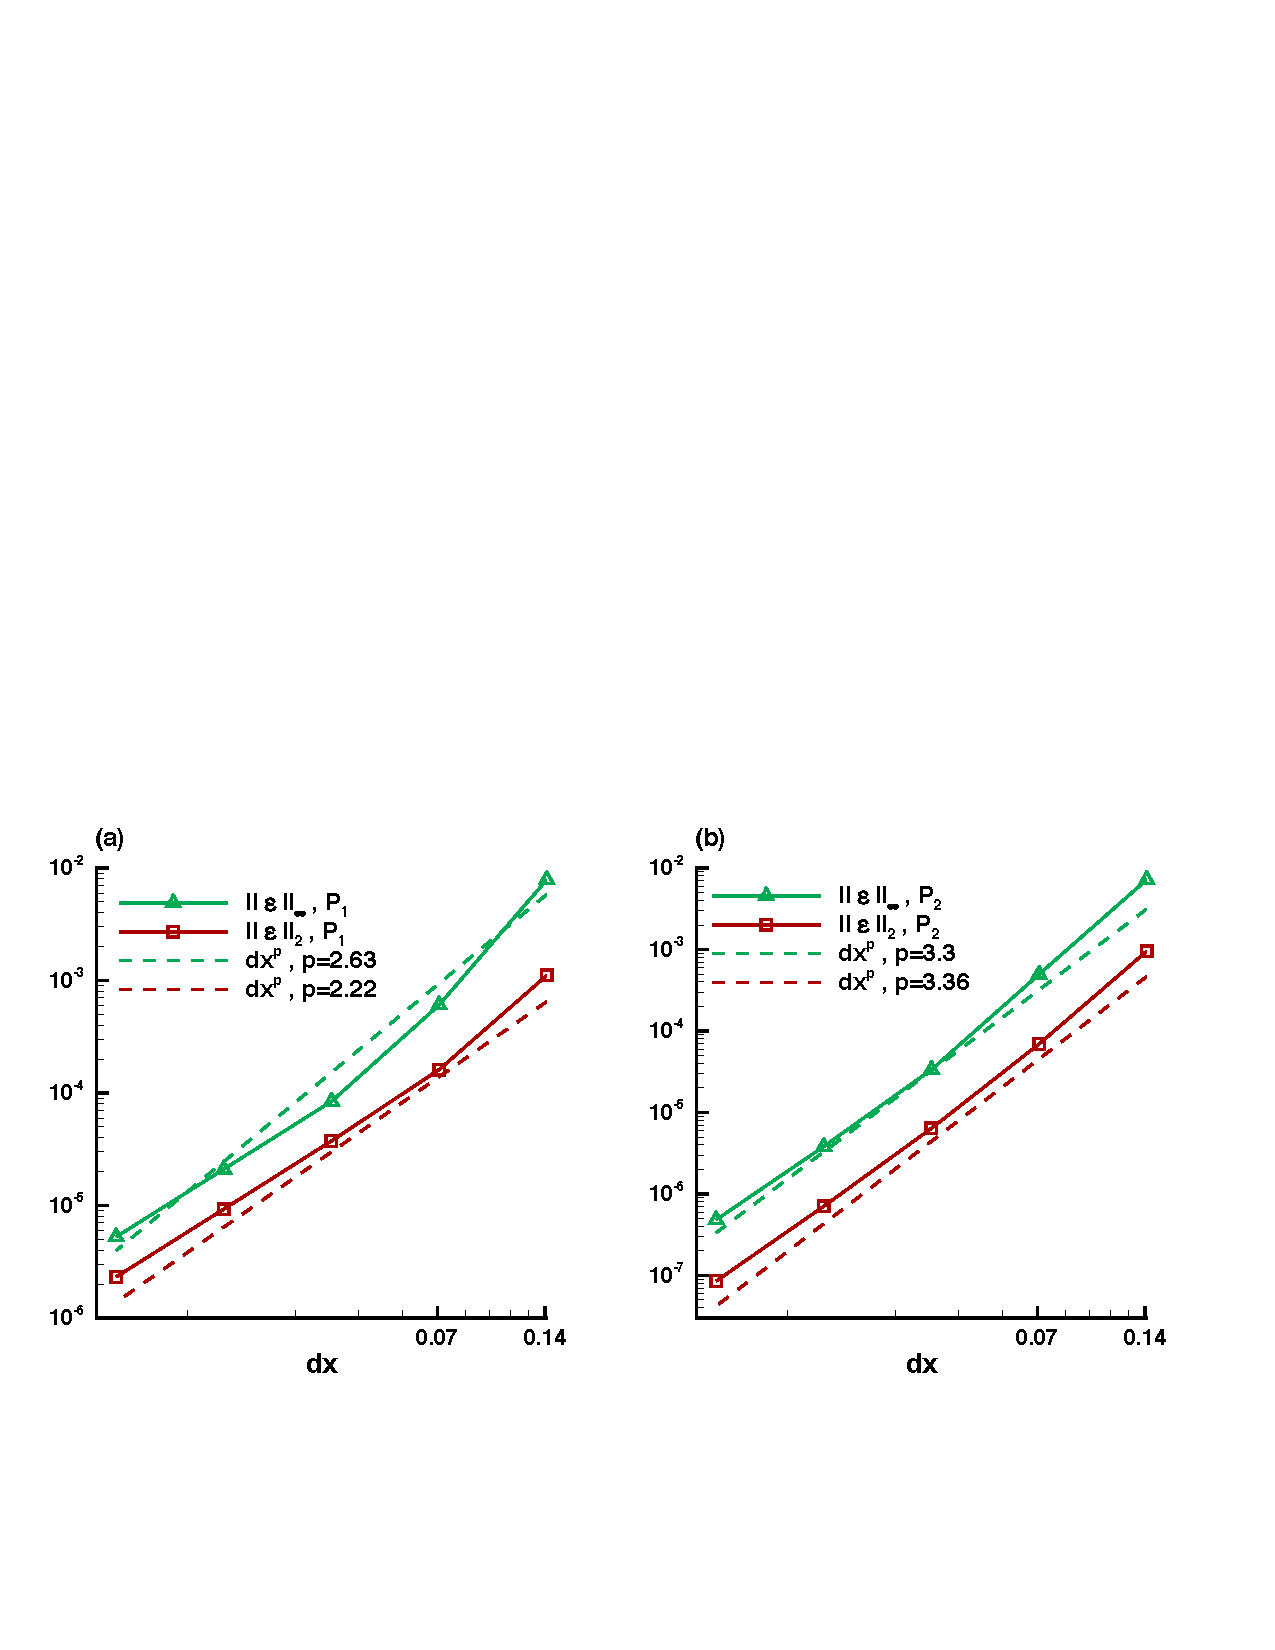
\includegraphics[width=0.98\textwidth]{\figpath/Fig_cap_2/Convergence_BURGGRAF} 
	\end{center}
	\caption{Burggraf flow. Evolution of the global error $\| \varepsilon_h \|$ for both $\mathcal{L}_2$-norm and $\mathcal{L}_\infty$-norm, with different grid size. A Taylor-Hood finite element (P$_2$ for velocity and P$_1$ for pressure) is used for space discretization by taking either P$_1$ finite element (a) or P$_2$ finite element (b) for the temperature field.}
	\label{fig-conv-burggraf}
\end{figure}

To demonstrate the space accuracy of our method, we compute the well-known analytical solution called the Burggraf flow.
It consists of a steady recirculating flow in a square cavity $[ 0 , 1] \times [ 0 , 1]$, with a moving wall at the top boundary and non-slip wall conditions at the others :

\begin{eqnarray}
   u(x,0) &=& u(0,y) = u(1,y) = 0, \\
   u(x,1) &=& \sigma (x^4 - 2x^3 + x^2).
\end{eqnarray}
Besides, constant temperatures are imposed at the top and the bottom walls, while others are assumed to be adiabatic.
The exact solution of the flow is:
\begin{eqnarray}
   u1(x,y) &=& \sigma g'(x) h'(y), \\\nonumber
   u2(x,y) &=& - \sigma g''(x) h(y), \\\nonumber
   p(x,y)   &=& \frac{\sigma}{Re} \left( h^{(3)}(y) g(x) + g''(x)h'(y) \right) + \frac{\sigma}{2} g'(x)^2 \left( h(y)h''(y)-h'(y)^2 \right),\\ \nonumber
   T(x,y) &=& T_{c} + (T_{h} - T_{c}) y + a(x) b(y), \\ \nonumber
\end{eqnarray}
with,
\begin{eqnarray}
   g(x) &=& \frac{x^5}{5} - \frac{x^4}{2} - \frac{x^3}{3}, \\ \nonumber
   h(y) &=& y^4 - y^2, \\ \nonumber
   a(x) &=& \cos (\pi x), \\ \nonumber
   b(x) &=& y(1-y).
\end{eqnarray}
Hence, forcing term are defined as follows:

\begin{eqnarray}
   f_{u1} &=& 0 \\ \nonumber
   f_{u2} &=& \sigma^2 h(y) h'(y) \left( g''(x)^2 - g'(x)g^{(3)}(x) \right) \\ \nonumber
   &+& \frac{\sigma}{Re}\left( g^{(4)}(x) h(y) + 2 g''(x)h''(y) + g(x) h^{(4)}(y) \right) \\ \nonumber
   &+& \frac{\sigma^2}{2} g'(x)^2 \left( h(y) h^{(3)}(y) - h'(y)h''(y) \right) - \frac{Ra}{Pr Re^2} T(x,y),\\ \nonumber
   f_T &=& u1(x,y) a'(x) b(y) + u2(x,y) \left( T_h - T_c + a(x) b'(y) \right) \\ \nonumber
   &-& \frac{K}{Re Pr} \left( a''(x)b(y) + a(x) b''(y) \right).
\end{eqnarray}
We use the Taylor-Hood finite element (P$_2$ for velocity and P$_1$ for pressure) for the space discretization with either P$_1$ or P$_2$ finite element for the temperature field.
Figure \ref{fig-conv-burggraf} plots the decrease of the global discretization error $\| \varepsilon_h \|$ for both $\mathcal{L}_2$-norm and $\mathcal{L}_\infty$-norm function of the grid size.
The expected second order convergence is obtained with a P$_1$ finite element for the temperature (Figure \ref{fig-conv-burggraf}a), and even a nearly third order is noticed with a P$_2$ finite element on the temperature (Figure \ref{fig-conv-burggraf}b).

\subsection{Manufactured solution} \label{subsub-conv-nourg}
\begin{figure}
	\begin{center}
		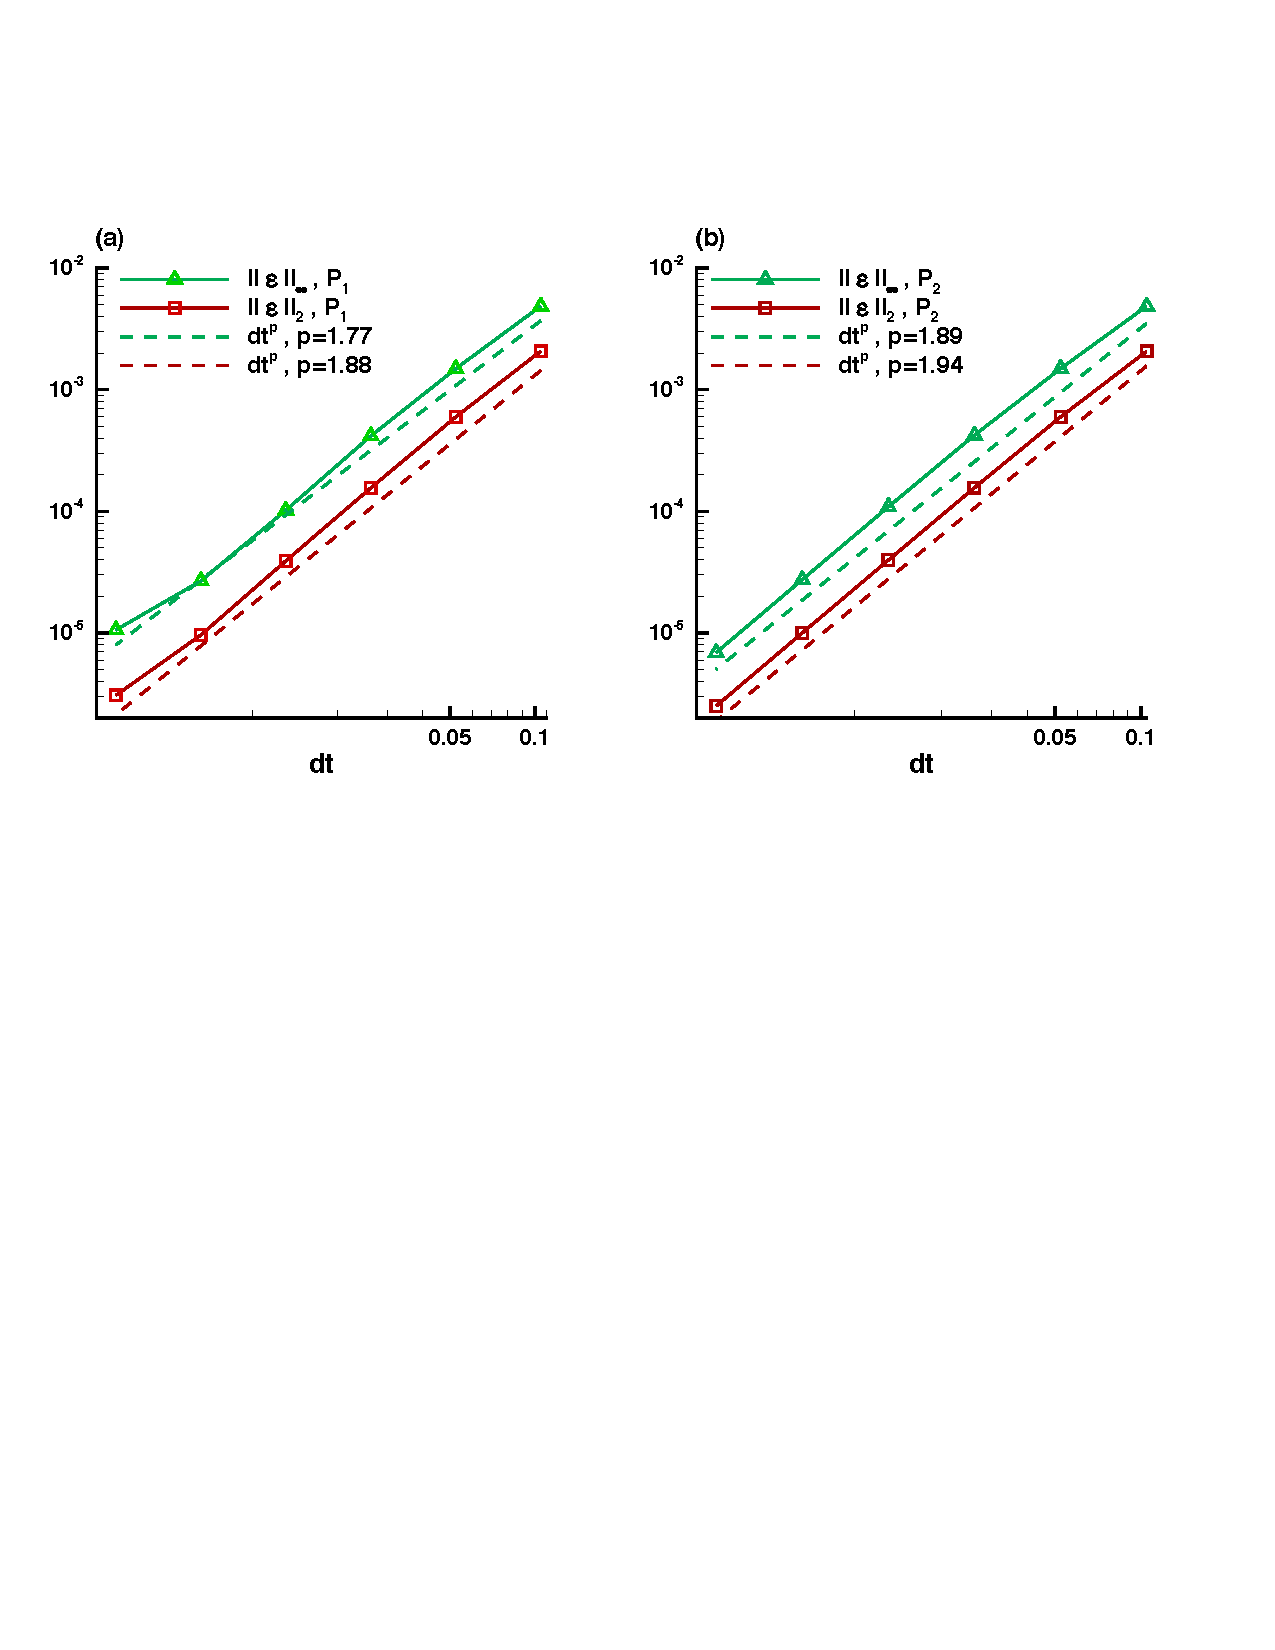
\includegraphics[width=0.98\textwidth]{\figpath/Fig_cap_2/Convergence_BDF2} 
	\end{center}
	\caption{Manufactured solution of \cite{nourgaliev2016fully} for unsteady incompressible Navier-Stokes equation at dimensionless time $t = \pi$. Evolution of the global error $\| \varepsilon_h \|$ for both $\mathcal{L}_2$-norm and $\mathcal{L}_\infty$-norm, with different time steps, with a P$_1$ finite element (a) and a P$_2$ finite element (b) for the temperature.}
	\label{fig-conv-bdf2}
\end{figure}

The time integration is based on the implicit second order scheme BDF2.
We use the manufactured solution of \cite{nourgaliev2016fully} to measure the temporal convergence order.
\begin{eqnarray}
	u_1(x,y,t) &=& \left( \delta U_0 + \alpha_u \, \sin(t) \right) \, \cos(x+ \gamma_1 t) \, \sin(y+ \gamma_2 t), \\ \nonumber
	u_2(x,y,t) &=& - \left( \delta U_0 + \alpha_u \sin(t) \right) \, \sin(x+ \gamma_1 t) \, \cos(y+ \gamma_2 t), \\ \nonumber
	T(x,y,t) &=& \bar{T} + \left( \delta T_0 + \alpha_t \sin(t) \right) \, \cos(x+ \gamma_1 t) \, \sin(y+ \gamma_2 t), \\ \nonumber
	p(x,y,t) &=& \bar{P} + \left(\delta P_0 + \alpha_p \sin(t) \right) \, \sin(x+ \gamma_1 t) \, \cos(y+ \gamma_2 t), 
\end{eqnarray}
The value of the constants are reported on Table \ref{tab-constant}.
\begin{table}[!h]
\centering
\begin{tabular}{*{10}{c}}
 % \toprule
  $\gamma_1$ & $\gamma_2$ & $\bar{P}$ & $\bar{T}$ & $\delta P_0$ & $\delta T_0$ & $\delta U_0$ & $\alpha_p$ & $\alpha_u$ & $\alpha_t$\\
   \midrule
  $0.1$ & $0.1$ & $0$ & $1.0$ &  $0.1$ & $1.0$ & $1.0$ & $0.05$ & $0.4$ & $0.1$ \\
 % \bottomrule

 \end{tabular}
\caption{Parameter for the manufactured solution.}
\label{tab-constant}
\end{table}

\noindent Thus, forcing terms are:

\begin{eqnarray}
	f_x &=& \alpha_u \, \cos(t) \, \cos(a) \sin(b) - U_c \, \gamma_1 \, \sin(a) \sin(b) + U_c \, \gamma_2  \, \cos(a)\cos(b) \\ \nonumber
	  & & - U_c \,  u_1(x,y,t) \, \sin(a) \sin(b) + U_c \,  u_2(x,y,t) \, \cos(a) \cos(b)
	  + P_c \, \cos(a) \cos(b)\\ \nonumber
	  & & + \frac{1}{Re} \, u(x,y,t), \\	  \nonumber
	f_y &=& - \alpha_u \,  \cos(t)  \, \sin(a) \cos(b) - U_c \,  \gamma_1  \,  \cos(a) \cos(b) + U_c \,  \gamma_2 \,  \sin(a)\sin(b) \\ \nonumber
		  & & - U_c \,  u_1(x,y,t)  \,  \cos(a) \cos(b) + U_c  \, u_2(x,y,t)  \,  \sin(a) \sin(b)
		  -  P_c  \,  \sin(a)  \,  \sin(b)\\ \nonumber
		  & & -\frac{1}{Re} \,  v(x,y,t)
		  - \frac{Ra}{Pr Re^2} \,  T(x,y,t), \\  \nonumber
	f_{\theta} &=& \alpha_t \,  \cos(t) \,  \cos(a) \sin(b) -  T_c  \,  \gamma_1 \,  \sin(a) \sin(b) + T_c \,   \gamma_2  \,  \cos(a)\cos(b) \\ \nonumber
		  & &-  T_c \,  u_1(x,y,t)  \,  \sin(a) \sin(b)  
		  +   T_c  \,  u_2(x,y,t)  \, \cos(a) \cos(b) 
		  + \frac{K}{Re Pr} \,  T_c  \, \cos(a) \sin(b), \\ \nonumber
\end{eqnarray}

with: 
$	U_c = (\delta U_0 + \alpha_u \sin(t)), \,
	T_c = (\delta T_0 + \alpha_u \sin(t)), \,
	P_c = (\delta P_0 + \alpha_u \sin(t)), $ \\
and $	a = (x+ \gamma_1 t), \,
	b = (y+ \gamma_2 t). \\$

Since the space convergence rate was evaluated in \S \ref{subsub-conv-burg}, we fixe the grid size to $dx = 0.01$ to ensure a small spatial discretization errors, and we vary decreasingly the time step.
Time convergence is displayed in Figure \ref{fig-conv-bdf2}. 
The evolution of the global error with different time steps is plotted for both  $\mathcal{L}_2$-norm (red line) and $\mathcal{L}_\infty$-norm (green line), and the expected second order convergence is exposed for both P$_1$ (Figure \ref{fig-conv-bdf2}a) and P$_2$ (Figure \ref{fig-conv-bdf2}b) finite element for the temperature.

\section{A finite-element toolbox for the simulation of phase-change systems with natural convection}\label{sec-desc-prog}

The methods described previously were implemented in a 2D toolbox based on FreeFem++ software.
Using two input files, the toolbox offers to the user the choice between three scalings in order to compute different physical systems involving natural convection flow, ranging from natural convection of air and water to melting and solidification cycle of PCM or water freezing.
The solutions can be saved at recurrent iterations defined by the user beforehand, allowing later to restart the computation from  saved solutions.
In this section we first describe the architecture of the programs and the organisation of files.
Then we focus on the list of input parameters and the structure of output files.

\begin{figure}
	\begin{center}
		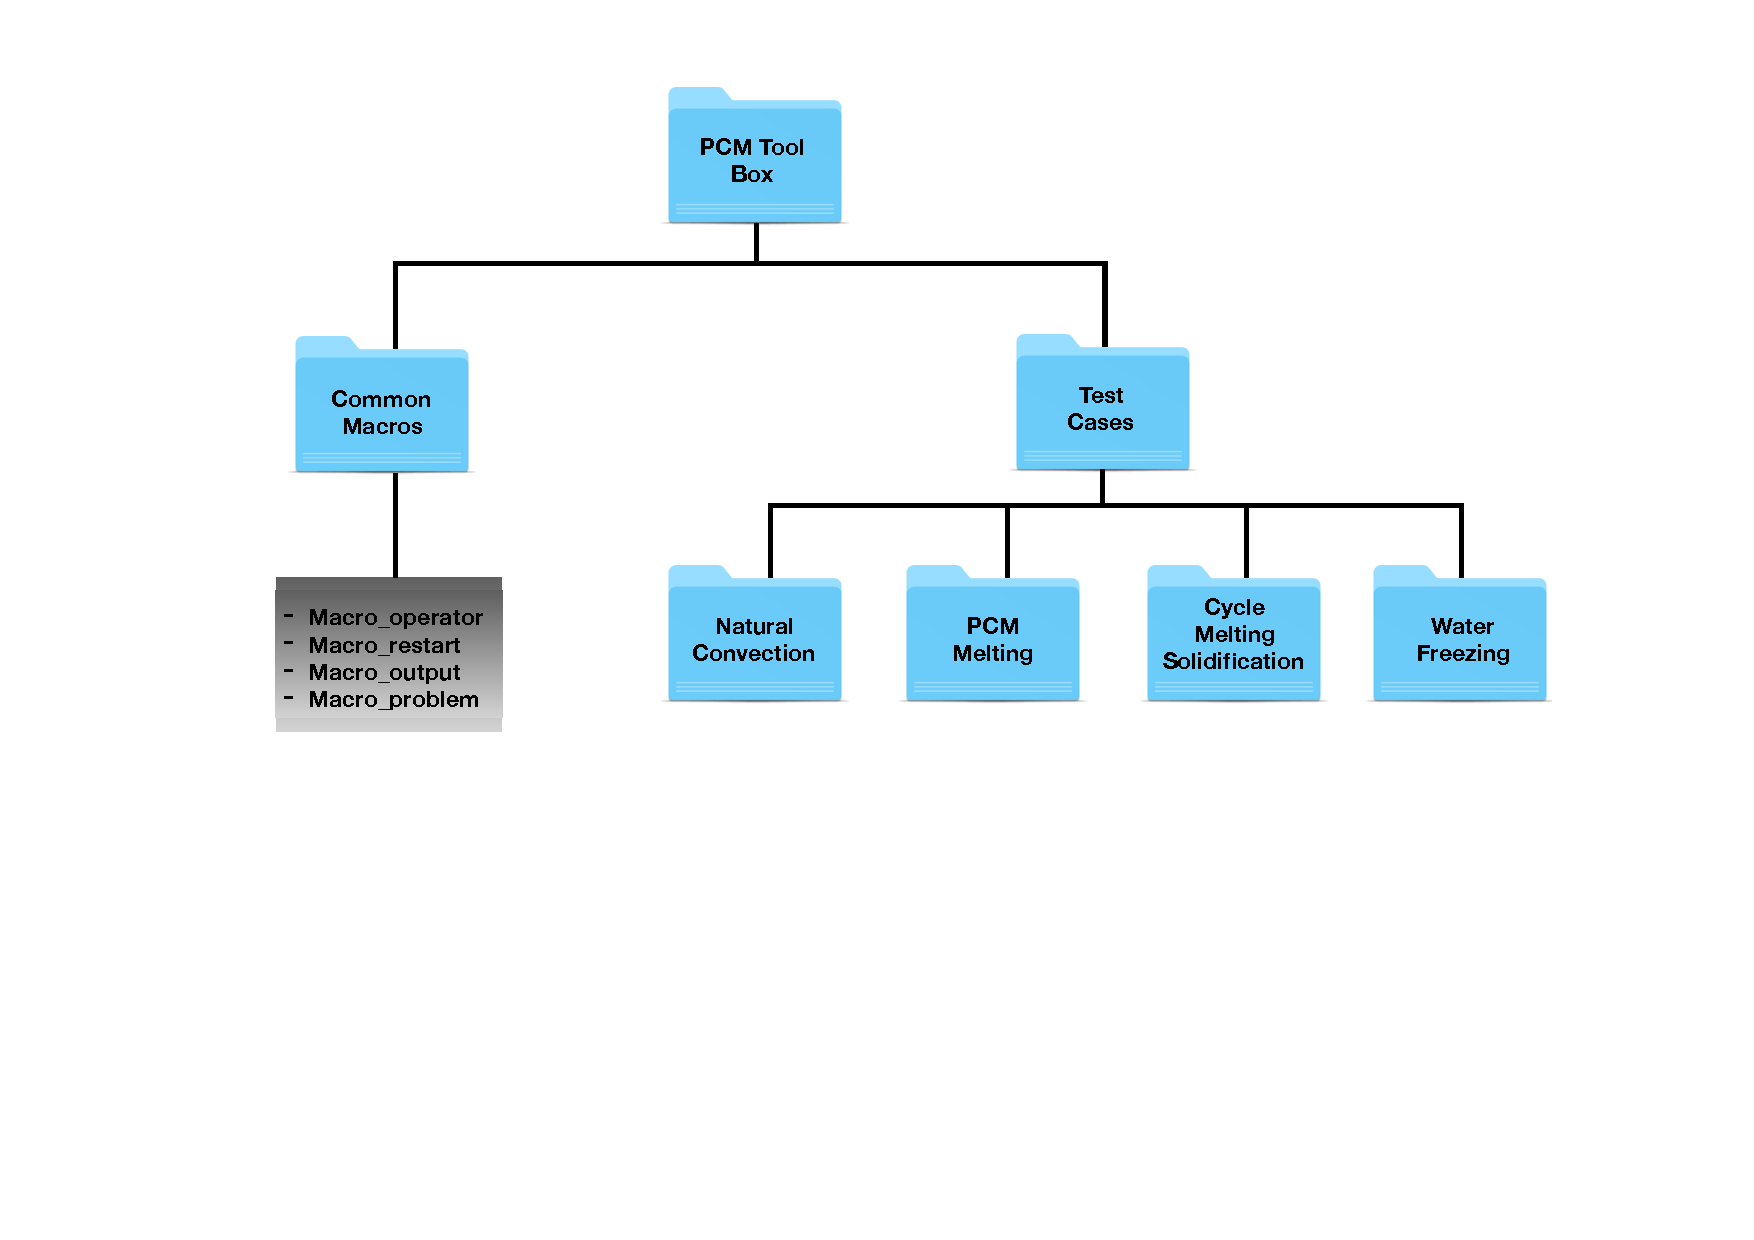
\includegraphics[width=0.9\textwidth]{\figpath/Fig_cap_2/FOLDER_arbor_2}
	\end{center}
	\caption{Folder tree structure of the FreeFem++ toolbox to solve phase change problems. Test cases and common macros are separated into two folders.}
	\label{fig-folder-tree}
\end{figure}

\subsection{Program architecture}
Figure \ref{fig-folder-tree} gives a schematic overview of the content of the toolbox. All files are provided in a directory called {\it "PCM ToolBox FreeFem"}. 
This directory is organized as follows:
\begin{enumerate}
   \item the {\em Common Macros} directory contains four files:
   \begin{itemize}
      \item {\em Macro$\_$operator.idp} contains all macros and functions related to mathematical operators,
      \item {\em Macro$\_$restart.idp} contains the scripts to be used to take the computation back from saved solutions,
      \item {\em Macro$\_$output.idp} contains the scripts allowing to output the solutions,
      \item {\em Macro$\_$problem.idp} contains the variational formulation of the problem. 
   \end{itemize}
   \item The {\em Test Cases} directory contains four subdirectories clustering different physical test cases, including the natural convection of air or water in a differentially heated square cavity, the melting of a PCM included in various containers, the melting-solidification cycle of a PCM and finally the freezing of pure water in a square cavity. 
   For all cited cases, three files are given for each subdirectories: {\em NEWTON$\_$\$case.edp} the main FreeFem++ script file, $param_\_phys.inc$ the physical parameters and $param_\_num.inc$ the numerical parameters.
   The natural convection case can be launched, for example, using the following command line in a terminal window:\\
  {\em FreeFem++ NEWTON$\_$airconv.edp -nbseg 80}.\\
  This will run the natural convection of air using $80 \times 80$ grids.
\end{enumerate}

\subsection{Input parameters}
We focus now on the description of the input parameters.
The physical parameters and parameters related to the run are separated into two files.\\
{\bf (1)} First, the file $param_\_phys.inc$ contains the physical descriptions of the problem:

\begin{itemize}
   \item {\bf typeT}: indicates the finite element type for the temperature. Choose between P$_1$ or P$_2$,
   \item {\bf scalAdim}: defines the characteristic scales of the problem. Choose between 1,2 or 3 \citep{dan-2014-JCP}:
   \begin{eqnarray} \label{eq-scal1}
    (1) &:&  V_\vref^{(1)} = \frac{\nu_l}{H} \Longrightarrow \ds t_\vref^{(1)} = \frac{H^2}{\nu_l}  \Longrightarrow \Rey=1,\\
      \label{eq-scal2}
     (2) &:& V_\vref^{(2)} = \frac{\alpha}{H} \Longrightarrow \ds t_\vref^{(2)} = t_\vref^{(1)} \Prd  \Longrightarrow \Rey =1/\Prd,\\
      \label{eq-scal3}
     (3) &:& V_\vref^{(3)} = \frac{\nu_l}{H} \sqrt{\frac{\Ray}{\Prd}} \Longrightarrow \ds t_\vref^{(3)} = t_\vref^{(1)} \sqrt{\frac{\Prd}{\Ray}}       \Longrightarrow \Rey = \sqrt{\frac{\Ray}{\Prd}},
\end{eqnarray}
   \item {\bf x$_0$, x$_l$, y$_0$, x$_l$}: correspond to the dimensions of the cavity.
   \item {\bf Pr, Ra, Ste}: are the dimensionless numbers Prandtl, Rayleigh and Stefan respectively defined in (\ref{eq-Rayleigh}) and (\ref{eq-RePr}),
   \item {\bf T$_{hot}$, T$_{cold}$}: denote the dimensionless temperatures according to (\ref{eq-adim}),
   \item{\bf bcu$_1$, bcu$_2$, bcT, bcp}: correspond to the velocity, the temperature and the pressure boundary conditions respectively.
   \item {\bf epsi}: expresses the half width $\varepsilon$ of the mushy region. \underline{Default value} = $0.01$,
   \item {\bf dt}: refers to the dimensionless time step,
   \item {\bf t$_{max}$}: fixes the dimensionless final time,
   \item {\bf Parameters for regularization functions}: \\
 Parameters of the hyperbolic-tangent function used to regularize the discontinuous parameters are set by default as follows:
 \end{itemize}
    \begin{table}[!ht]
    \centering
    \begin{tabular}{*{8}{c}}
     & {\bf f$_{{\hbox {\tiny S}}}$} & {\bf f$_{{\hbox {\tiny L}}}$} & {\bf as} & {\bf $\theta s$} & Rs & {\bf C$_{{\hbox {\tiny MUSHY}}}$} & {\bf b$_{{\hbox {\tiny MUSHY}}}$} \\
       \toprule
       {\it Enthalpy} & 0 & 1/Ste & 1 & 0.01 & 0.01  & - & - \\
       \midrule
       {\it Carman - Kozeny} & 0 & 1 & 1 & 0.01 & 0.01  & 10$^6$ & 10$^{-7}$ \\
          \midrule
       {\it Conductivity (water)} & 1 & 2.26/0.578 & 1 & $\theta_f$ & 0.015 & - & - \\
       \bottomrule
     \end{tabular}
    \label{tab-constant}
    \end{table}
   \begin{itemize} 
    \item {\bf rho(T) and Drho(T)}: refer to the density-temperature coupling model (water case): 
    $\rho(T) = \rho_m (1 - \omega | T - T_m |^q)$. The constants take the value:
    \begin{table}[!ht]
    \centering
    \begin{tabular}{*{4}{c}}
    $\rho_m$ [kg/m$^3$]  & $\omega$ [$^o$C$^{-q}$] & q & $T_m$  [$^o$C] \\
       \toprule
            $999.972$ & $9.2793 \cdot 10^{-6}$ & $1.894816$ & $4.0293$ \\
       \bottomrule
     \end{tabular}
    \label{tab-rho}
    \end{table}
    \item {\bf f$_B$(T), df$_B$(T)}: correspond to the buoyancy force.% in the Boussinesq approximation.
    \end{itemize}
\noindent {\bf (2)} Second, the file {\em param$\_$num.inc} contains the parameters relying on the run:\\
{\bf Restart Parameters:}
\begin{itemize}
   \item {\bf Nsave}: indicates the output recurrence of the solutions. $N\!save = 1$ would save the solution for all iterations.
   \item {\bf Nrestart}: indicates the recurrence to save meshes and solutions,
   \item {\bf Ncondt}: enables a clean stop. The solutions are saved before stopping the current run after {\it Ncondt} iterations,
   \item {\bf Nremesh}: corresponds to the mesh adaptation recurrence. The value of $1$ should adapt the mesh at every time steps,
   \item {\bf IFrestart}: corresponds to the initial state. 
   $I\!Frestart = 0$ means that the computation starts from fully solid initial condition for melting (resp. fully liquid for solidification) while other positive values allow to restart from previous saved solutions. 
   Furthermore, a negative value corresponds to a specific initial condition: steady state solution for example.
\end{itemize}
{\bf Newton parameters:}
\begin{itemize}
   \item {\bf epsconv}: corresponds to the precision criterion for steady cases,
   \item {\bf gamma}: is the penalty parameter in the continuity equation (\ref{eq-time-disc1}). \underline{Default value} = $10^{-7}$,
   \item {\bf tolNewton}: fixes the Newton tolerance $\xi_N$ (see (\ref{eq-Newton-algo})). \underline{Default value} = $10^{-6}$,
   \item {\bf newtonMax}: limits the maximum iteration $k$ of the Newton algorithm in (\ref{eq-Newton-algo}). \underline{Default value} = $50$,
   \item {\bf a$_1$, a$_2$, a$_3$}: represent the BDF scheme coefficients. a$_1 =1$, a$_2 = 1$, a$_3 = 0$ would correspond to the first order and a$_1 =1.5$, a$_2 = 2$, and a$_3 = 0.5$ to the second order scheme.
\end{itemize}
{\bf Mesh building parameters:}
\begin{itemize}
   \item {\bf nbseg}: sets the number of point along the $x$ and $y$ directions,
   \item {\bf errh}: fixes the interpolation error level. \underline{Default value} = $0.01$,
   \item {\bf hmin, hmax}: give the minimum and the maximum edge size respectively,
   \item {\bf adaptratio}: is the ratio for a prescribed smoothing on the metric. For a value less than $1.1$ no smoothing is done. \underline{Default value} = $1.8$,
   \item {\bf nbvx}: limits the number of vertices generated by the mesh generator. \underline{Default value} = $9000$.
\end{itemize}

\noindent {\bf Output parameters:}
   \begin{itemize}
      \item {\bf dircase}: corresponds to the name of the output folder,
      \item {\bf fcase}: corresponds to the name of the main ouput file.
   \end{itemize}

\subsection{Output parameters}
When a computation starts, the output directory is created.
It contains a set of Tecplot files whose name includes the prefix (defined by the parameter {\bf fcase}), the current iteration and the current dimensionless time $t$. 
The solutions can be read by either Tecplot software or any other CFD Visualization tools (Paraview, Visit, etc.).
Moreover, {\em .gmsh}  and {\em RST} files necessary for restarts are also generated in the output directory.
This directory will additionally contain an {\em .echo} file with a summary of the main parameters, informations on the run and the names of the output files and a copy of the input parameters allowing an easy reproducibility of each runs.


%%%%%%%%%%%%%%%%%%%%%%%%%%%%%%%%%%%%%%%%%%%%%%%%%%%%%%%%%%%
\section{Numerical resolution for large scale simulation}

\subsection{Domain decomposition method with FreeFem++: FFDDM}
Solving the Navier-Stokes-Boussinesq equation in a three dimensional configuration can generate a large problem size.
The natural convection of air in a cube of dimensions $[0,1]^3$ with $40 \times 40 \times 40$ grids involve $3$ millions of unknowns in the linear system.
For such a large size of problem, memory lack issue can rapidly arise with sequential algorithms.
It is thus essential to distribute date among several processors.
A natural approach is the domain decomposition method.

FFDDM (FreeFem++ Domain Decomposition Method) is a parallel part of FreeFem++ allowing to use parallel solver in FreeFem++.
The data distribution among the processor is done via an overlapping domain decomposition and a related linear algebra.
The linear system is then solved by using the domain decomposition method as preconditioners to the GMRES Krylov method.

We use in our simulations the Optimized Restricted Additive Schwarz (ORAS) preconditionner.
To solve the linear equation $A x = rhs$, the ORAS preconditionner reads:
\begin{equation}
   M_{RAS}^{-1} = \sum_{j=1}^{\mathcal{N}} R^T_j D_j (R_j A R^T_j)^{-1} R_j,
\end{equation}
$R_j$ denote the restriction operators and $D_j$ are square diagonal matrices.
Local matrices are defined as:
\begin{equation}
   A_j = R_i A R_i^T.
\end{equation}
The duplicated unknowns due to the overlap between subdomains are coupled via a partition of unity:
\begin{equation}
   I = \sum_{i=1}^{\mathcal{N}} R_i^T D_i R_i
\end{equation}
Thus, the global solutions $U$ is defined as:
\begin{equation}
  U = \sum_{i=1}^{\mathcal{N}} R_i^T D_i R_i U =  \sum_{i=1}^{\mathcal{N}} R_i^T D_i U_i
\end{equation}

\subsection{Strong scalability experiment with ffddm} \label{sub-scal-ffddm}
We assess here the strong scalability of the ORAS preconditioner on the 3D differentially heated cube cavity.
We vary the number of subdomains while the global system size is fixed.
With a P$_2$ finite element for the temperature, we solve $7.2$ million of unknowns (d.o.f).
The subdomain is decomposed into subdomains with METIS, ranging from $48$ to $400$ subdomains.
Fig. \ref{fig-scalability} illustrate the evolution of the total wall clock time for different subdomains, in which a good speed up is observed.
From $48$ to $320$ we observe a linear speed up. 
The total runtime passes from $2$ hours for $48$ subdomains to $15$ minutes for $320$ subdomains.
The linear speed up is then slightly lost for $400$ subdomains but remains reasonable.
In Tab. \ref{tab-scalability} we detail the timing relative to this test.
The column "Factorization" denotes the time spent in the factorization of the local submatrices and "GMRES" gives the time taken by GMRES to solve the global linear system
by the domain decomposition algorithm.

\begin{figure}%[!htbp]
\begin{minipage}{\linewidth}
\begin{center}
 {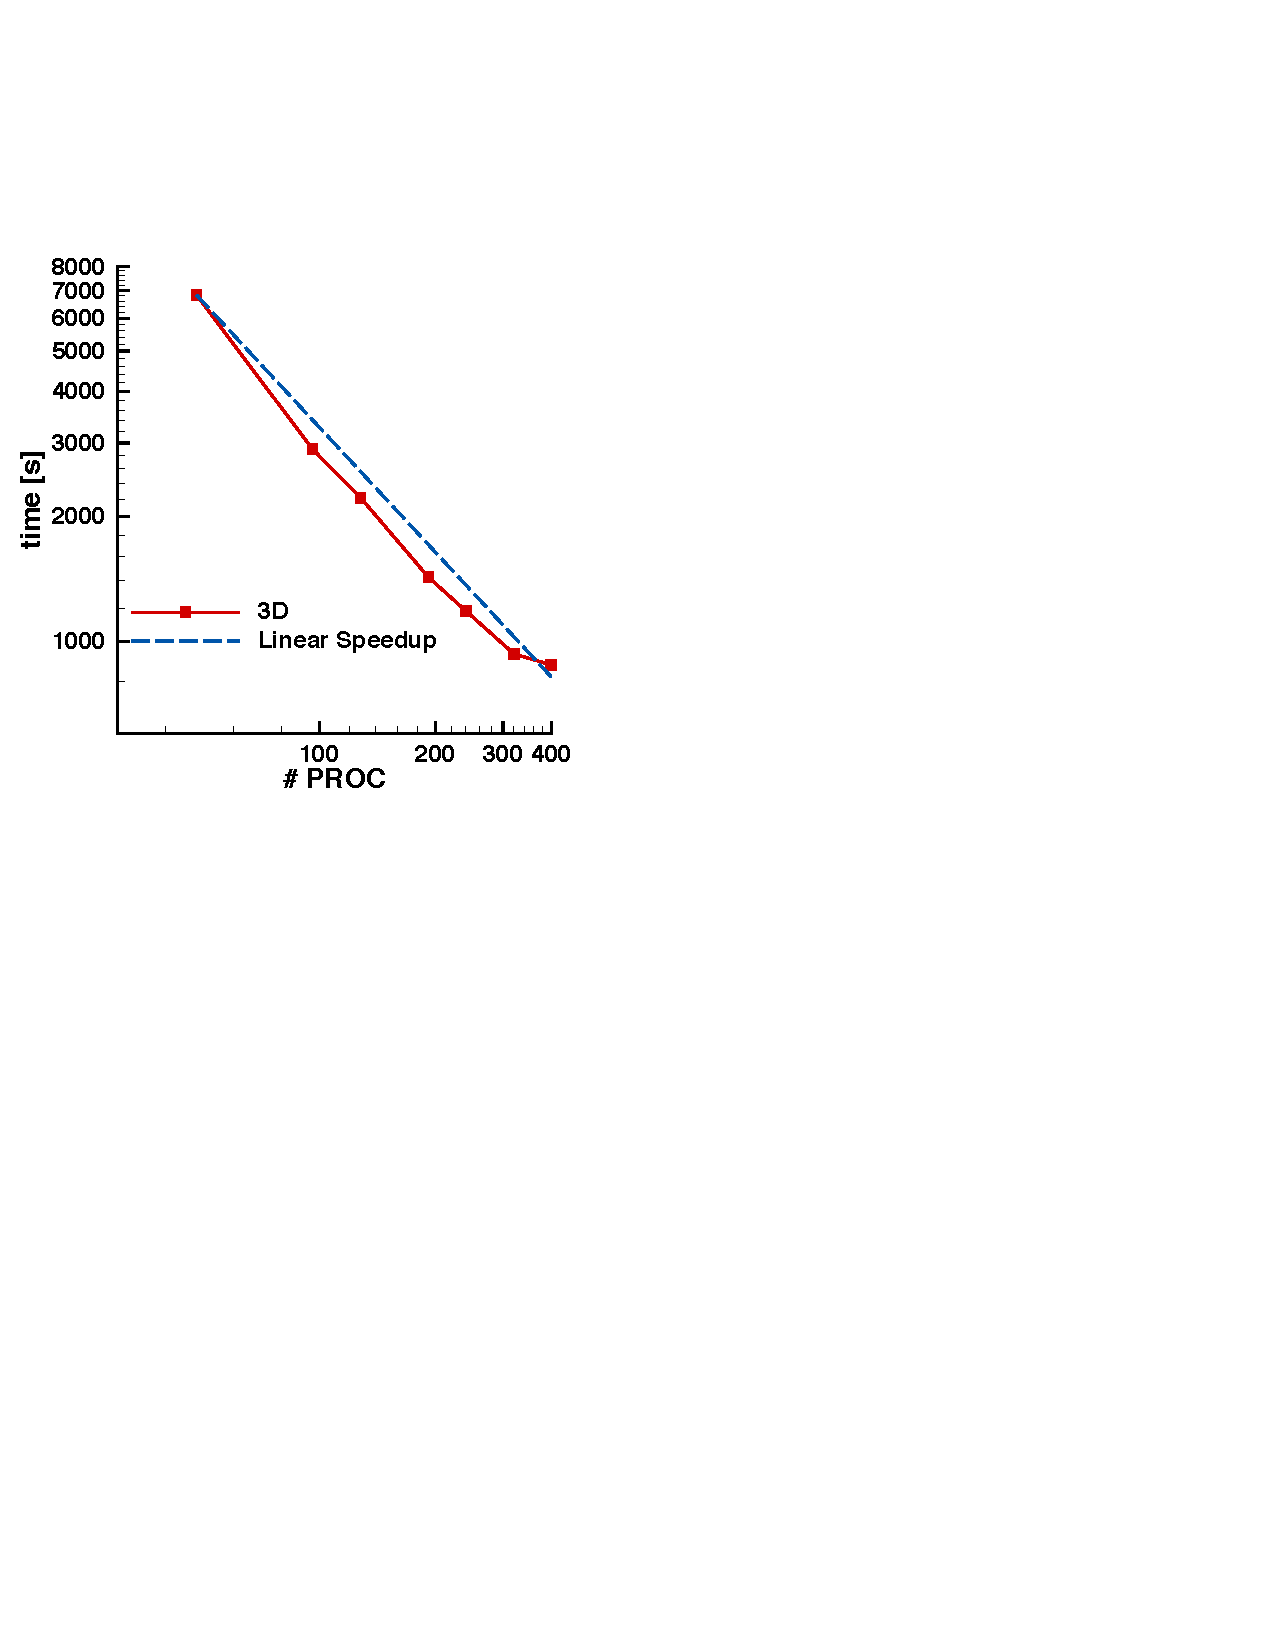
\includegraphics[width=.45\textwidth]{\figpath/Fig_cap_natconv/Scal_ffddm_2level}}
 {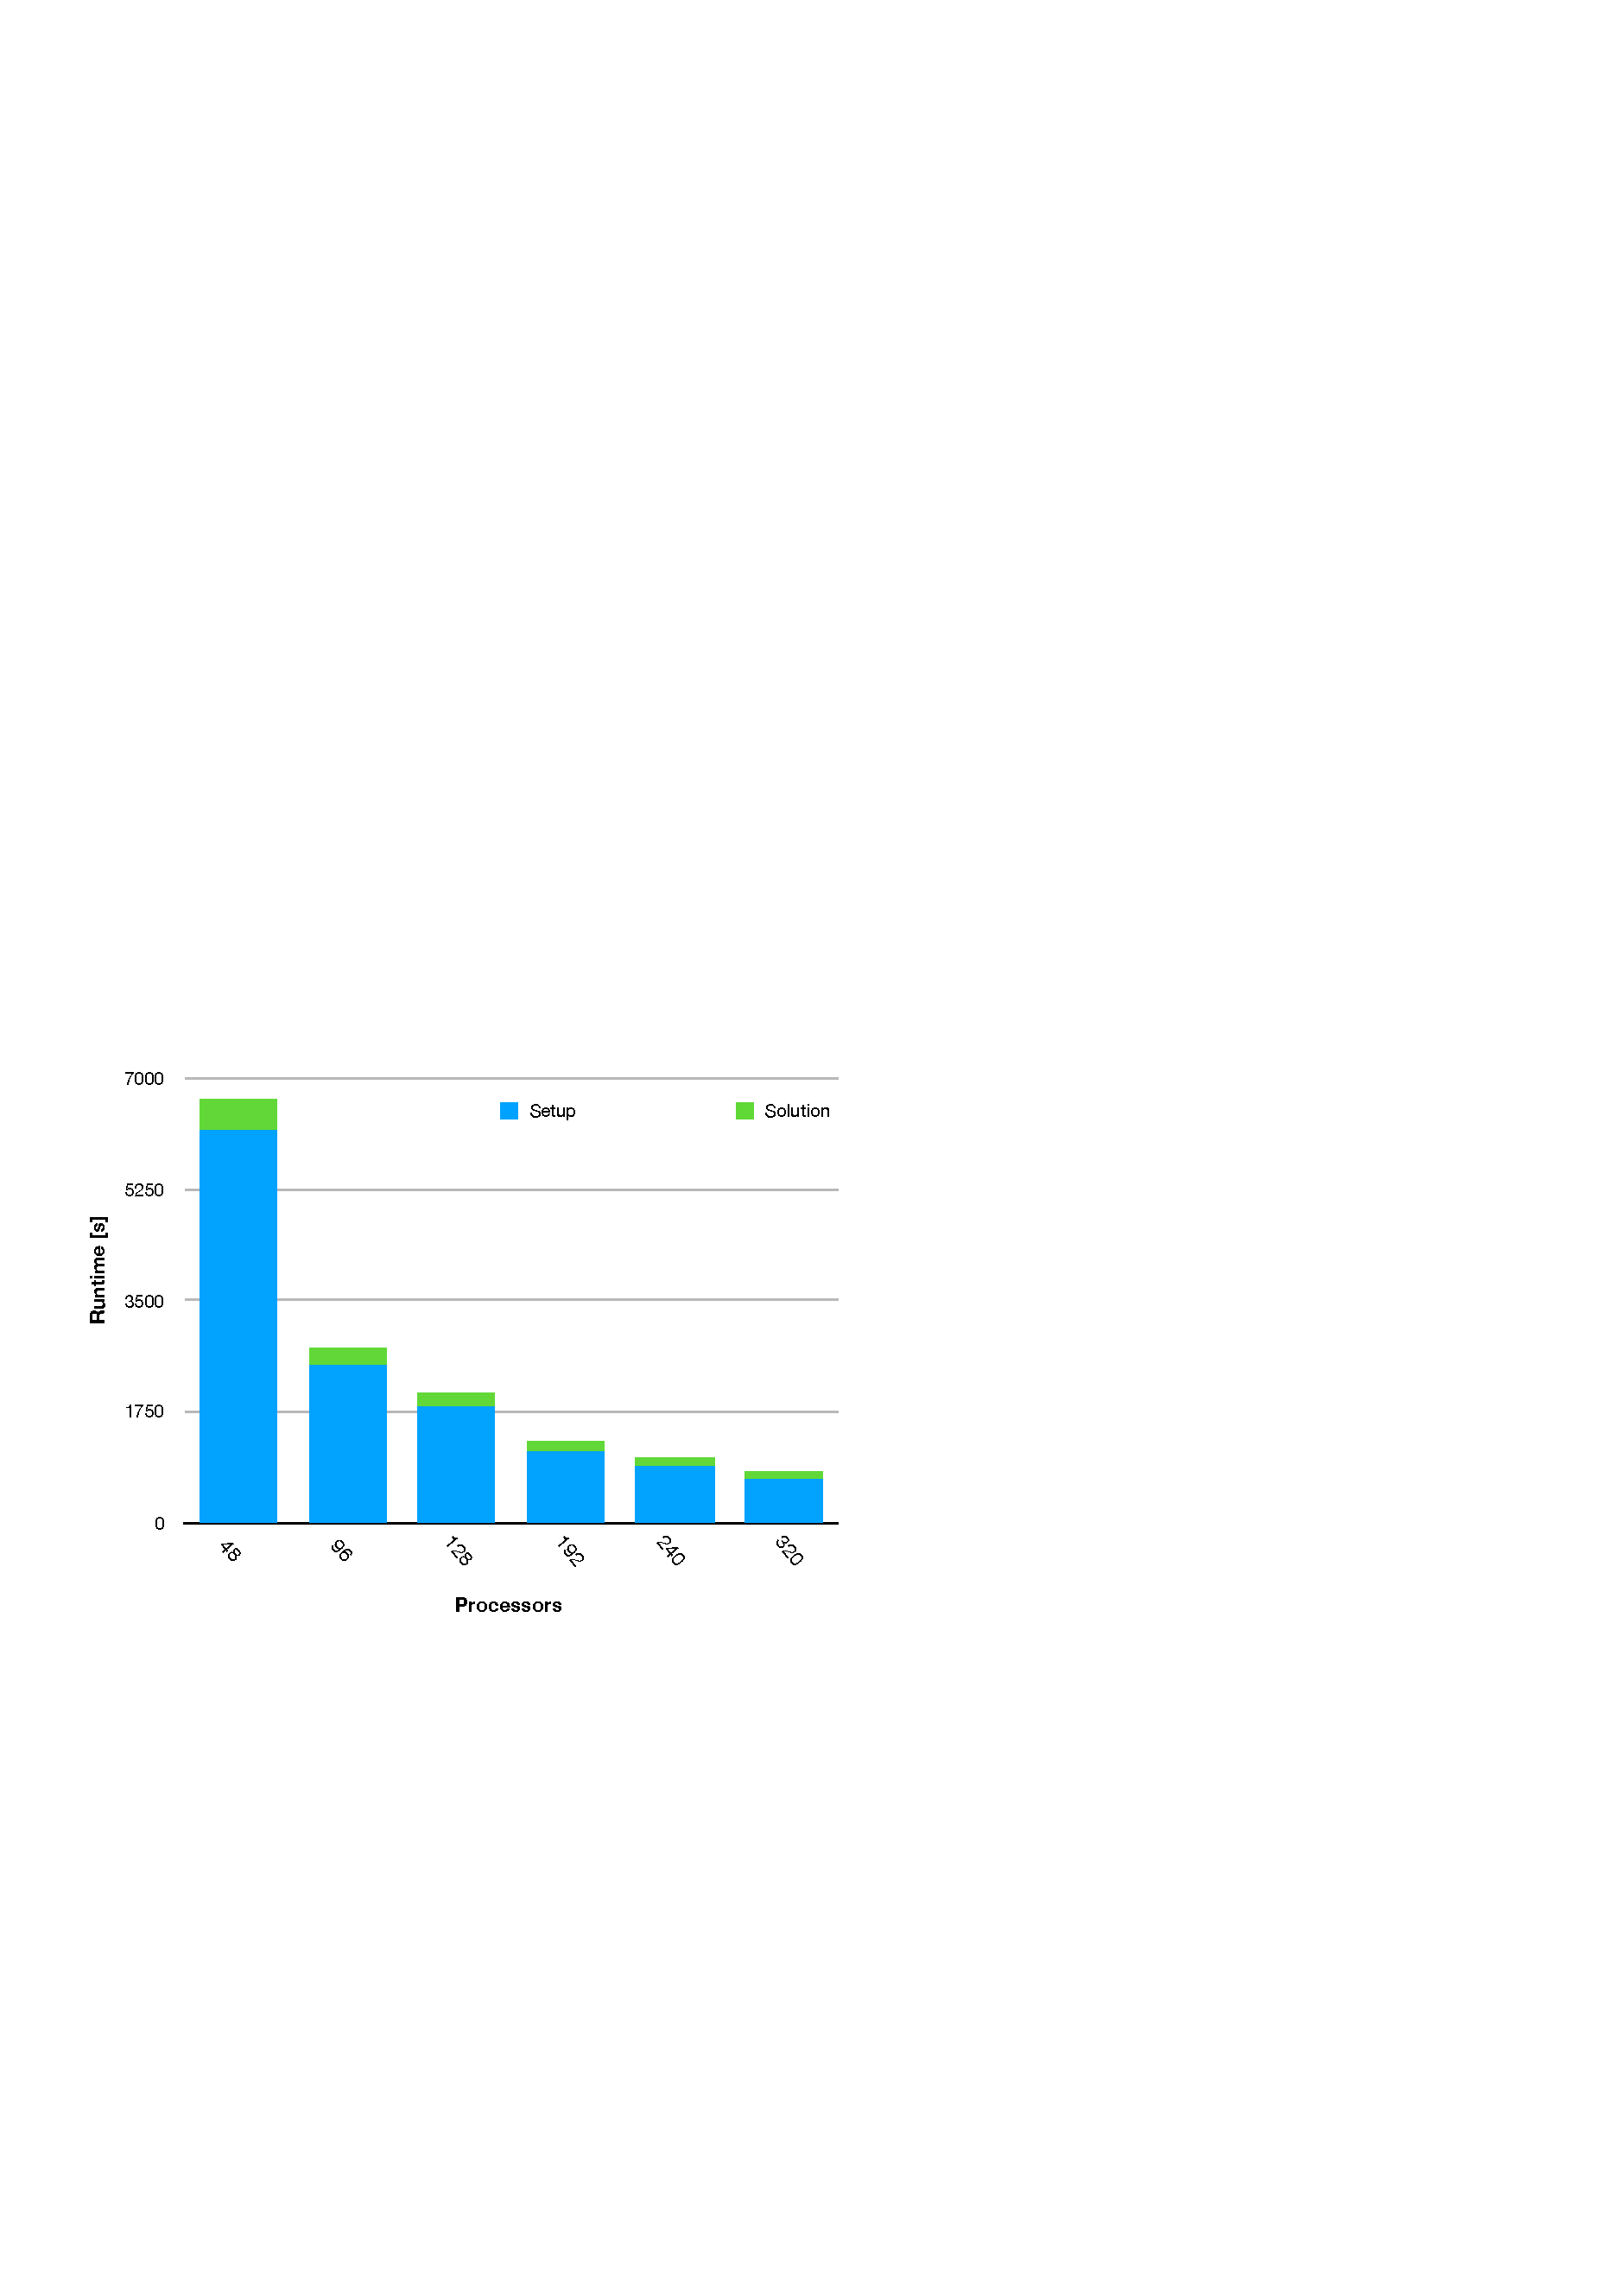
\includegraphics[width=.5\textwidth]{\figpath/Fig_cap_2/scal_ffddm_P2}}
\end{center}
\end{minipage}
\caption{Strong scalability of the ORAS preconditioner: $7.2$ millions of d.o.f and subdomains ranging from $48$ to $400$.}
\label{fig-scalability} 
\end{figure}

\begin{table}[!h]
	\begin{center}
		\begin{tabular}{cccc}
			 $\mathcal{N}$ & Factorization (s)  & GMRES (s)  & Total Step (s) \\ \hline \hline
			 48 & 6186.33  & 473.66  &  6659.99 \\
			 96 & 2468.68  & 283.099 &  2751.779 \\
			 128 & 1814.26 &  237.853 &   2052.113\\
			 192 & 1111.5  &   169.174 &  1280.674 \\
			 240 & 889.422  & 146.539 &  1035.961\\
			 320 & 674.204   &  114.346 & 788.55 \\
			 400 & 614.418  &  107.422 &  721.84\\ \hline
		\end{tabular}
	\end{center}
	\caption {Strong scaling experiment in 3D differentially heated cavity. $7.2$ millions of d.o.f and subdomains ranging from $48$ to $400$. }
	\label{tab-scalability}
\end{table}


